\subsection{Methodology}
        We apply the so-called transcript method to solve our (OCP).
    This schemes' main idea consists of transforming the underlying problem of
    optimizing functional governed by a differential equation into a
    finite-dimensional optimization problem with restrictions. To fix ideas,
    let $x$, $u$ denote state and control and consider the optimal
    control problem
    \begin{equation*}
        \begin{aligned}
                & \min J(x(\cdot), u(\cdot)) = g_0(T, x(T))
                & \text{Functional cost}
            \\
                & \dot{x} = f(t, x(t), u(t)),
                \quad\forall t \in [0, T],
                & \text{Dynamics}
            \\
                & u(t) \in \mathcal{U}[0, T] \text{for a.e. } t\in [0, T]
                & \text{Admisible controls}
            \\
                & g(x(t), u(t)) \leq 0
                & \text{Paht constrain}
            \\
                & \Phi(x(0), x(T)) = 0
                & \text{Boundary conditions}.
        \end{aligned}
    \end{equation*}
        Then, transcription methods transform this infinite-dimensional
    optimization problem into a finite dimension problem (NLP) via
    discretization of dynamics, state, and control.  For example, if we
    employ the Euler method with a discretization of $N$ constant steps with
    size $h$, then we can solve
    \begin{equation}
        \label{eqn:nlp}
        \begin{aligned}
                & \min g_0(t_N, x_N)
            \\
                &
                    x_{i+1} = x_i + h f(x_i, u_i),
                &
                    i = 0, \dots, N - 1
            \\
                &
                    u_i \in \mathcal{U},
                &
                    i = 0, \dots, N
            \\
                &
                    g(x_i, u_i) \leq 0,
                &
                    i = 0, \dots, N
            \\
                &
                    \Phi(x_0, x_N) = 0,
                &
                    i = 0, \dots, N
            \\
            \text{where} &
            \\
                &
            x_i \approx x(t_i),
            \qquad
            u_i \approx u(t_i)
            \\
            &
            \left\{
            t_0 = 0,\quad
            t_i = i h \ (i=1,\dots, N-1),\quad
            t_N = T
            \right\}.
        \end{aligned}
    \end{equation}
    Let $Y = \{x_0, \dots, x_N, u_0,\dots u_N\}$.
    Thus \Cref{eqn:nlp} defines a nonlinear programming problem on the
    discretized state and control variables of the form
    \begin{equation}
        \label{eqn:nlp_form}
        \begin{aligned}
            &
            \min F(Y)
        \\
        \text{such that} &
        \\
            &
            LB \leq C(Y) \leq UB .
        \end{aligned}
        %\tag{NLP}
    \end{equation}
    %
        The numerical analysis and design of transcript methods is a well
    established  and active research numerical field. There is a baste
    literature about robust methods and resently it apperars implementations in
    vogue languages like Julia
    \cite{DunningHuchetteLubin2017, LubinDunningIJOC}, Python \cite{libcmaes},
    Matlab \cite{matlabOpt}, and others. We refer the reader to
    \cite{Betts2001,Seywald1993} for a more systematic discussion.

        Our simulations rely on the \verb|Bocop| package
    \cite{Bocop,BocopExamples} to solve our (OCP). Bocop is part of the
    development of the INRIA-Saclay initiative for open source optimal control
    toolbox and supported by the team Commands. BOCOP solves the NLP problem in
    \Cref{eqn:nlp_form} by the well known software \textsc{Ipopt} and using
    sparse exact derivatives computed by ADOL-C.

        We provide in \cite{gitHub} a GitHub repository with all regarding R
    and Bocop sources for the sake of reproductivity. This repository also
    encloses data sources and python code to reproduce all reported figures.

\subsection{Simulation of hypothetical scenarios}
        We follow the guidelines reported by the WHO Strategic Advisory Group
    of Experts (SAGE) on Immunization Working Group on COVID-19 Vaccines
    modeling questions presented in \cite{sage2020}. According to this SAGE's
    document, we simulate scenarios to illustrate vaccination policies'
    response with a preventive vaccine. We aim to contrast the impact of the
    burden of COVID-19 mitigation regarding
    \begin{enumerate}[(\textbf{SCN}-1)]
        \item Optimal versus constant vaccination policies
        \item Vaccine efficacy
        \item Induced vaccine immunity
        \item Natural immunity
    \end{enumerate}

        We consider vaccine profiles\textemdash efficacy and induced vaccine
    immunity in concordance with the expected but still unconfirmed data
    \textemdash from the firms Cansino-Biologics, Astra Zeneca, and Pfizer.
    Further, since reinfection and induced vaccine immunity parameters remain
    unavailable, we see pertinent explore the effect of plausible settings.
    \Cref{tbl:scene_parameters} enclose a brief description and parameter
    values regarding each scenario. The reader can also access the web
    \verb|Chart Studio Graph| of each figure regarding data and
    \verb|plotly| \cite{plotly} visual representation.
%
    \begin{table*}[b]
        \centering
        \begin{tabular}{%
                >{\centering}
                p{0.1\textwidth}
                p{0.23\textwidth}
                p{0.57\textwidth}
            }
            \toprule
            \textbf{Simulation Scene}
            & \textbf{\qquad Description}
            & \textbf{Set-up} \quad
            $(x_{coverage}, T, \epsilon, \delta_V^{-1}, \delta_R^{-1})$
            \\
            \midrule
            \textbf{(SCN-1)}
            &
            Likening between optimal and constant
            vaccination policies.
            &
            (%
            \SI{20}{\percent},
            \SI{180}{days},
            \SI{70}{\percent},
            \SI{730}{days},
            \text{lifelong}
            )
            \\
            \textbf{(SCN-2)}
            &
            Vaccine efficacy blow
            &
            (%
            \SI{50}{\percent}, %
            \SI{365}{days}, %
            $\left\{
            \SI{50}{\percent},
            \SI{70}{\percent},
            \SI{90}{\percent}
            \right\}
            $, %
            \SI{180}{days}, %
            \SI{730}{days}
            )
            \\
            \textbf{(SCN-3)}
            &
            Induced vaccine immunity period
            &
            (%
            \SI{50}{\percent}, %
            \SI{365}{days}, %
            \SI{90}{\percent},
            $\left\{
            \SI{365}{days},
            \SI{730}{days}
            \right\}
            $, %
            \SI{365}{days}%
            )
            \\
            \textbf{(SCN-4)}
            &
            Natural immunity period
            &
            (%
            \SI{50}{\percent}, %
            \SI{365}{days}, %
            \SI{90}{\percent}, %
            \SI{730}{days}, %
            $
            \left\{
                \SI{90}{days},
                \SI{180}{days},
                \SI{365}{days}
            \right\}
            $%
            )
            \\
            \bottomrule
        \end{tabular}
        \caption{
            Setup parameters for counterfactual and response scenarios. See
            \Cref{tbl:fixed_parameters} for the rest of parameters.}
        \label{tbl:scene_parameters}
    \end{table*}
%
To perform the simulations corresponding to the scenarios presented in
\Cref{tbl:scene_parameters}, we fix the values for the set of parameters
presented in \Cref{tbl:fixed_parameters-OCM}.
%
\begin{table}[tbh]
    \begin{center}
        \begin{tabular}{rc@{}c}
            \toprule
            \multicolumn{3}{c}{\textbf{Parameters values}}
            \\
            \midrule
            \\
                & \multicolumn{2}{c}{\textbf{(SCN-1)--(SCN4)}}
                \\
                \cmidrule{2-3}
                \\
                $\beta_S$
                & \multicolumn{2}{l}{\num{0.363282}}
            \\
                $\beta_A$
                & \multicolumn{2}{l}{\num{0.251521}}
            \\
                $\alpha_{S}$
                & \multicolumn{2}{l}{\num{0.0925069}}
            \\
                $\alpha_{A}$
                & \multicolumn{2}{l}{\num{0.167504}}
            \\
                $\delta_{E}$
                & \multicolumn{2}{l}{\num{0.196078}}
            \\
                $\mu$
                &\multicolumn{2}{l}{\num{0.0000391389}}
            \\
                $\theta$
                & \multicolumn{2}{l}{\num{0.11}}
            \\
                $p$
                & \multicolumn{2}{l}{\num{0.1213}}
            \\
                $a_D$
                & \multicolumn{2}{l}{\num{7.5}}
            \\
                $a_S$
                & \multicolumn{2}{l}{\num{0.008418473}}
            \\
                $\kappa$
                & \multicolumn{2}{l}{\num{0.05}}
            \\
                $B$
                & \multicolumn{2}{l}{\num{9500}}
            \\
            \\
                & \textbf{(SCN-1)}
                & \textbf{(SCN-2)}--\textbf{(SCN-4)}
            \\
                \cmidrule{2-3}
                %\cmidrule{3-3}
            %\\
%                \cmidrule{3-3}
%            \\
            $\lambda_{V}$
                & \num{0.00123969}
                & \num{0.00189903}
            \\
                $u_{min}$
                & \num{-0.000619845}
                & \num{-0.00094952}
            \\
                $u_{max}$
                & \num{0.00619845}
                & \num{0.00474758}
            \\
            \bottomrule
        \end{tabular}
        \caption{%
            Fixed parameters values of system in
            \Cref{eqn:optimal_control_problem}.}
        \label{tbl:fixed_parameters-OCM}
    \end{center}
\end{table}
%
\section*{Optimal Versus Constant Vaccination Policies: (SCN-1)}
        To fix ideas, we display in
        \Cref{fig:lifelongvaccinationpolicies,%
        fig:lifelongvaccinationpoliciesOutbreak}
    the counterfactual scenario regarding no intervention, constant vaccination
    policy (CP), and optimal vaccination policy (OP) with a vaccine profile of
    efficacy $\epsilon = \SI{70}{\percent}$, and induced immunity
    $\delta_V^{-1} = \SI{180}{days}$ and over a campaign for \SI{20}{\percent}
    of coverage at \SI{180}{days}. \Cref{fig:lifelongvaccinationpolicies}
    suggests that the OP improves CP vaccination policy response according to
    the burden disease due to mortality, morbidity, and coverage time.
    \Cref{fig:lifelongvaccinationpoliciesOutbreak} confirms this improvement by
    comparing symptomatic reported cases, saving lives, and the disease dynamics
    without vaccination. Although both campaigns use the same number of vaccine
    doses and the same vaccine profile, we observe that OP implies fewer deaths
    and symptomatic cases.

        \Cref{fig:lifelongvaccinationpolicies}, shows a scenario where
    $R_0>1$. Despite $R_V$
    remains below but close to
    $R_0$, vaccination reproductive number
    $R_V$, could
    explain vaccination response with constant policies according
    to the mitigation factor
    \begin{equation}
        \label{eqn:mitigation_factor}
        \left(
            1 -
        \frac{\epsilon \lambda_V}{\mu+\delta_V+\lambda_V}
        \right).
    \end{equation}
    That is,  disease mitigation is strongly related to vaccine efficiency
    $\epsilon$ and vaccination rate $\lambda_V$. Further, given a dynamic with
    not vaccine intervention and $\mathcal{R}_0>1$, $\mathcal{R}_V$ suggests a
    minimal vaccination rate to drive this dynamic to the disease-free state
    but subject to vaccines with particular efficacy.
%
    \begin{figure*}[tbh!]
        \centering
        \includegraphics[scale=0.6, keepaspectratio]{%
            LifeLongVaccinationPolicies.png%
        }
        \caption[Effect of the vaccination policy on the burden COVID-19]{%
        Effect of the vaccination policy on the burden COVID-19.
        (A) vaccination policies' response regarding constant vaccination rate
        and optimal modulated in the burden of COVID-19 quantified in DALYs.
        Blue translucent color corresponds to policies with constant
        vaccination rate x. Green tone denotes the vaccination optimal
        modulated rate. For contractual reference, gray shade represents the
        burden of COVID-19 without vaccination. (B) evolution of the
        vaccination covering according to each policy, the optimal policy
        requires less time to reach 20 percent of the vaccinated population.
        (C) vaccination schedule for each vaccination policy.
        See \href{https://plotly.com/~sauldiazinfante/131/}{%
                https://plotly.com/~sauldiazinfante/131/}
        for plotly visualization and data.
        }
        \label{fig:lifelongvaccinationpolicies}
    \end{figure*}
    \begin{figure*}[tbh!]
        \centering
        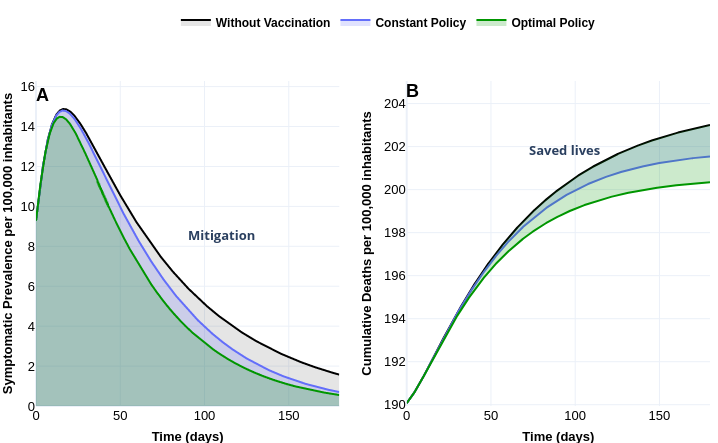
\includegraphics[scale=0.6,
        keepaspectratio]{LifeLongVaccinationPoliciesOutbreak.png}
        \caption[Effect of the vaccination policy on outbreak evolution.]{
        Effect of the vaccination policy on outbreak evolution.
        (A) Optimal vaccination policy reaches a better response in mitigating
        symptomatic cases than a policy with a constant vaccination rate.
        (B) Shaded translucent regions denote the number of saved lives per
        \SI{100000}{inhabitants} according to constant (blue) or
        optimal modulated vaccination rates. Since the
        areas overlap, we note that optimal vaccination policy improves the
        number of saved lives. Data and web visualization in
        \href{%
            https://plotly.com/~sauldiazinfante/135/
        }{https://plotly.com/~sauldiazinfante/135/}.
        }
        \label{fig:lifelongvaccinationpoliciesOutbreak}
    \end{figure*}
%
\section*{Vaccine Efficacy (SCN-2)}
    In the authors words of press releases
    \begin{quotation}
      \say{%
          Pfizer says early analysis shows its Covid-19 vaccine is
          more than \SI{90}{\percent} effective \cite{cnn_health_2020}.%
        }

      \say{%
       Russia says its Sputnik V COVID-19 vaccine is \SI{92}{\percent} effective
      \cite{reuters2020}.}
    \end{quotation}
    This is a game changer fact\textemdash FDA would accept a vaccine of
    \SI{50}{\percent}. Following this sort of ideas,
    \Cref{fig:efficiencyvaccineprofile,fig:efficiencyvaccineprofileOutbreak}
    displays the response of the optimal vaccination policy according to three
    vaccines with different efficacy. \Cref{fig:efficiencyvaccineprofile}-A
    displays the burden COVID-19 in DALYs for vaccines with
    efficacy of \SI{50}{\percent}, \SI{70}{\percent}, \SI{90}{\percent}.
    According with a time horizon of \SI{1}{year} and coverage of
    \SI{50}{\percent}, \Cref{fig:efficiencyvaccineprofileOutbreak} display an
    improvement of at least tree times in prevalence of symptomatic cases and
    saved lives respect to the uncontrolled outbreak.
    \Cref{fig:efficiencyvaccineprofileOutbreak} reflects this
    effect in the prevalence of symptomatic cases (A) and in the number
    of saved lives shaded by the traslusent green color (B).
%
%-------------------------------------------------------------------------------
% Vaccine efficacy gradient
%
    \begin{figure*}[htb]
        \centering
        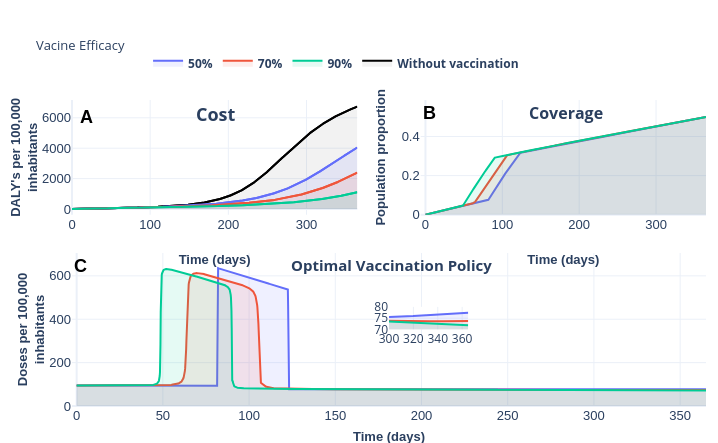
\includegraphics[scale=.60, keepaspectratio]{%
            ./EfficiencyVaccineProfile.png%
        }
        \caption[The response of COVID-19 on vaccine efficacy]{
            The response of COVID-19 burden on vaccine efficacy.
            (A) COVID-19 burden response quantified in DALYs per 100,000 to
            vaccines with efficacy of \SI{50}{\percent} (blue),
            \SI{70}{\percent} and \SI{90}{\percent}(red).
            (B) Coverage evolution to reach \SI{50}{\percent} of the total
            population vaccinated.
            (C) Optimal vaccination doses schedule according to the
            different efficacies. See
            \href{https://plotly.com/~sauldiazinfante/85/}{%
                https://plotly.com/~sauldiazinfante/85/} for
            visualization and data.
        }
        \label{fig:efficiencyvaccineprofile}
    \end{figure*}
%
    \begin{figure*}[htb]
        \centering
        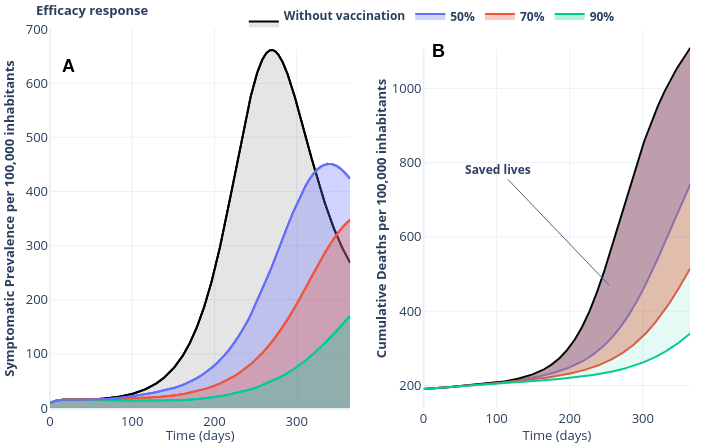
\includegraphics[scale=.6, keepaspectratio]{%
            ./EfficiencyVaccineProfileOutbreak.png%
        }
        \caption[Optimal Vaccination Policy]{
            (A) Effect of vaccine-efficacy of
            \SI{50}{\percent} (blue), \SI{70}{\percent}
             and \SI{90}{\percent} (red) on prevalence
             of symptomatic cases per SI{100000}{inhabitants}.
            (B) Effect of vaccine-efficacy on the number of saved lives.
            See
            \href{https://plotly.com/~sauldiazinfante/100/%
            }{https://plotly.com/~sauldiazinfante/100/} for data and
            visualization.
        }
        \label{fig:efficiencyvaccineprofileOutbreak}
    \end{figure*}

\section*{Vaccine-induced immunity (SCN-3)}
    Vaccine response also is strongly related with its induced
    immunity\textemdash parameter that at today remains well understood
    \cite{Jeyanathan2020}.
    Here we contrast two vaccines with different induced immunity. Let
    denote by $vax_1, vax_2$ vaccines with induced immunity capacity of one and
    two years respectively and common efficacy of \SI{70}{\percent}. Consider a
    vaccine camping of time horizon of one year and \SI{50}{\percent} coverage.
    Taking the same dynamics parameters, that is initial conditions, and base
    line parameters as in  \Cref{tbl:fixed_parameters} we explore a
    contrafactual scenario with an uncontrolled outbreak of
    $R_0 = \num{1.79493}$ and two controlled dynamics according to vaccines
    $vax_1$, $vax_2$. Thus, according to this immunity parameters and factor
    defined in \Cref{eqn:mitigation_factor}, respectively results
    $R_V^{[vax_1]} = \num{1.13913}$, $R_V^{[vax_2]} = \num{0.86756}$
    for vaccine immunities periods of one and two years. We display in
    \Cref{fig:induced_immunity_vaccine_profile} the regarding response of the
    vaccines $vax_1$ and $vax_2$. Since in this setting time
    horizon is of one year, the optimal policies follows similar schedules and
    implies similar gains in the number of years of life lost. Despite this
    similarities, \Cref{fig:inducedimmunity_vaccine_outbreak}
    displays in panel A a dramatically gain respect to the
    uncontrolled outbreak\textemdash since
    $R_V ^{[vax_1]}$ is near to one, prevalence fall-down more than five times
    and because $R_V ^{[vax_2]}$ is lest that one, prevalence of symptomatic
    cases tends to zero with damped oscillations.
    \Cref{fig:inducedimmunity_vaccine_outbreak} also endorses this gain,
    note that saved lives is represented by  shaded region with translucent
    and overlapped red blue colors.
%
%-------------------------------------------------------------------------------
% Induced vaccine immunity gradient
    \begin{figure*}[htb]
        \centering
        \includegraphics[scale=0.6, keepaspectratio]{%
        InducedImmunityVaccineProfile%
        }
        \caption[
            Effect of Vaccine-induced immunity effect on the burden of COVID-19.
        ]{
            (A) Effect on the burden of COVID-19 quantified in DALYs per
            \SI{100000}{inhabitants} due to vaccine-induced immunity of
            \SI{365}{days}(red) and 730 days (blue).
            (B) Coverage evolution to reach \SI{50}{\percent} of the total
            population vaccinated.
            (C) Optimal vaccination doses schedule according to the different
            vaccine-induced immunities. Since the time horizon is
            \SI{350}{days}, both policies follow similar profiles in coverage
            and schedule. Visualization and data in
            \href{https://plotly.com/~sauldiazinfante/111/}{%
                https://plotly.com/~sauldiazinfante/111/}.
        }
        \label{fig:induced_immunity_vaccine_profile}
    \end{figure*}
    %
    \begin{figure*}[htb]
        \centering
        \includegraphics[scale=0.6,keepaspectratio]{%
            InducedImmunityVaccineProfileOutbreak%
        }
        \caption[
           Effect of vaccine-induced immunity on mitigation and saved lives of
           COVID-19 outbreak]{
            (A) Effect of vaccine-induced immunity on mitigation of symptomatic
            prevalence per \SI{100000}{inhabitants}.
            (B) Number of saved lives. Since the reproductive vaccine number
            for the immunity of \SI{365}{days} results in \num{1.13913} and
            \num{0.86756} for \SI{730}{days}, this behavior is consistent.
            See \href{https://plotly.com/~sauldiazinfante/123/}{%
                https://plotly.com/~sauldiazinfante/123/}
            for data and visualization.
        }
        \label{fig:inducedimmunity_vaccine_outbreak}
    \end{figure*}
%-------------------------------------------------------------------------------
\section*{Natural Immunity Hypothesis (SCN-4)}
%
    ``Second infections raise questions about long-term immunity to
    COVID-19 and the prospects for a vaccine'', reported
    Heidi Ledford in \cite{Ledford2020b}. Following this line, we
    display in \Cref{%
            fig:natural_recovering_profile,%
            fig:natural_recovering_outbreak} the regarding response
    of a vaccine with \SI{90}{\percent} efficacy and
    contrasting with  natural immunity periods of
    \SI{90}{days}, \SI{180}{days}, \SI{365}{days}. Here,
    the adjective "natural" denotes the immunity that an individual
    develops after recovering from a previous bout of COVID-19. When natural
    immunity last one year, the burden of COVID-19 fall-down until
    around 120 DALYs. We confirm this behavior in the prevalence of
    symptomatic cases and cummulative deaths, as displayed in
    \Cref{fig:natural_recovering_outbreak}, when
    natural immunity is \SI{365}{days} the gain in mitigation respect to a
    natural immunity of \SI{90}{days} is at least and 100 times, while the
    number of deaths with a natural immunity of \SI{90}{days} reach 845 cases
    per \SI{100000}{inhabitants}, in contrast, of \SI{206} when natural
    immunity is \SI{365}{days}. Thus this simulation suggest that natural
    immunity plays a important role in the behavior of the controlled
    outbreak, which is consistent with the conclusions reported in
    \cite{Jeyanathan2020}.
%
    \begin{figure*}[tbh!]
        \centering
        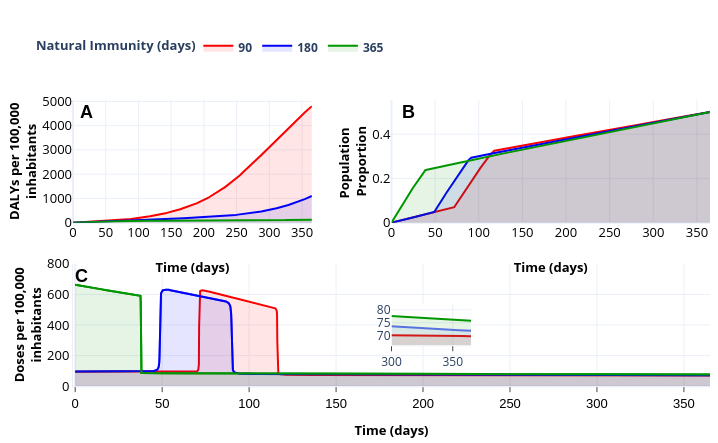
\includegraphics[scale=0.6,
        keepaspectratio]{NaturalRecoveringProfile}
        \caption[Effect of natural immunity on the burden of COVID-19]{
            (A) Effect on the burden of COVID-19 quantified in DALYs per
            100,000 inhabitants due to natural immunity of 90 days (red) and
            180 days (yellow) 365 days (green).
            (B) Coverage evolution to reach \SI{50}{\per} of the total
            population vaccinated.
            (C) Optimal vaccination doses schedule according to the different
            natural immunities.
            \href{https://plotly.com/~sauldiazinfante/95/}{%
                https://plotly.com/~sauldiazinfante/95/}
        }
        \label{fig:natural_recovering_profile}
    \end{figure*}
%
    \begin{figure*}[h!]
        \centering
        \includegraphics[scale=0.6, keepaspectratio]{%
            NaturalRecoveringProfileOutbreak%
        }
        \caption[Vaccine induced immunity profile.]{
            (A) Effect of  immunity on mitigation of
            symptomatic prevalence per 100,000 inhabitants.
            (B) Number of saved lives. Since the reproductive vaccine number
            for the immunity of 365 days results in \num{1.13913} and
            \num{0.86756} for \SI{730}{days}, this behavior is consistent.
            Plotly visualization and data in
            \href{https://plotly.com/~sauldiazinfante/104/}{%
                https://plotly.com/~sauldiazinfante/104/
            }.
        }
        \label{fig:natural_recovering_outbreak}
    \end{figure*}